\documentclass{article}
\usepackage{blindtext}
\usepackage[utf8]{inputenc}
\usepackage[T2A]{fontenc}
\usepackage[russian]{babel}
\usepackage{indentfirst}
\usepackage{amsmath}
\usepackage{hyperref}
\usepackage{graphicx}

\title{Онлайн оптимизация параметров рекомендательной системы}
\author{Александр Лактионов, МФТИ, ФИВТ, 497}
\date{Февраль, 2018}
\pagestyle{headings}

\begin{document}
 
\maketitle

\section{Задача}
\subsection{Постановка задачи}
Рекомендательные системы могут быть основаны на алгоритмах машинного обучения, бизнес-правилах и их комбинации. В большинстве случаев процесс создания модели, которая предсказывает интересные пользователю объекты, состоит из трёх частей:

\begin{enumerate}  
\item Подготовка, фильтрация и обработка данных 
\item Обучение модели
\item Предсказание рекомендаций для пользователя
\end{enumerate}

В модели может быть большое количество гиперпараметров – переменных, значения которых не оптимизируются в процессе обучения. Такие переменные делятся на два типа: те, которые подбираются до и после обучения модели. 
\par
В случае оффлайн-обучения раз в сутки, онлайн-оптимизация гиперпараметров для обучения не представляет большого интереса – новые точки в пространстве параметров будут проверяться очень долго. Параметры, которые можно изменить в процессе предсказания, напротив, могут быть оптимизированы в процессе работы алгоритма. 
\par
В данной работе рассмотрена оптимизация гиперпараметров, которые подбираются в процессе предсказания рекомендаций.
 

\subsection{Значимость задачи}
Рекомендательные системы используются в большом количестве сервисов и помогают пользователям находить ту информацию, которая им интересна. Рекомендации особенно полезны в сфере продаж в интернете, так как позволяют повысить конверсию в целевое действие. 
\par 
В данной работе рассматривается рекомендательная система для популярного сайта объявлений об аренде и продаже недвижимости в России. Детали реализации данного подхода изложены в тезисах [1]

\subsection{Применение в рекомендательной системе}
Рассматривается блок рекомендаций «Похожие объекты», расположенный на странице объявления, содержащий 5 объявлений, интересных пользователю и связанных с рассматриваемым объектом на странице 
\par 

\vspace{3mm}


\includegraphics[height=3cm]{img0.png}
\par
\vspace{3mm}

\subsubsection{Бизнес-правила}

В случае пользовательских сервисов нередко возникают продуктовые требования, выполнить которые невозможно, ограничившись только работой с моделью. Некоторые из подобных правил:
\begin{itemize}  
\item Не рекомендовать объекты из других категорий недвижимости (например, продажу новостройки к аренде офиса)
\item Не рекомендовать объекты из других регионов
\item Не рекомендовать объекты без фотографий
\end{itemize}

Подобные правила параметризуются индикаторами их использования. 

\subsubsection{Информация про контент}
Нередко про объекты известна дополнительная информация, которую можно использовать для модификации функции скоринга перед определением 5 наиболее интересных объектов. 
\par
Эта информация можно обновляться очень часто и может быть не учтена во время обучения модели:
\begin{itemize}  
\item Оценка объекта и аккаунта владельца модераторами сайта
\item Популярность объекта
\end{itemize}


\subsubsection{Влияние контекста}
При просмотре страницы объявления пользователь выражает свой интерес к данному объекту. Однако помимо этого есть много информации про самого пользователя, его поведение и просмотренные им объекты в прошлом.

\begin{itemize}  
\item Вес истории пользователя
\item Вес информации про просматриваемый объект
\end{itemize}


\subsubsection{Технические параметры}
В рассматриваемой рекомендательной системе используется поисковый движок ElasticSearch, в котором документы хранятся распределённо и по шардам. 
\par
При параллельном поиске похожих на историю пользователя или объект объявлений существует возможность досрочно прекратить запрос в рамках шарда, как только внутри него было найдено определенное количество документов. По умолчанию этот параметр равен бесконечности, однако если найти приемлимое значение, скорость работы всей системы можно увеличить в несколько раз. 

\begin{itemize}  
\item es.search: terminate\_after
\end{itemize}

\par
Значение оптимизируемой метрики можно сделать зависимым от времени работы алгоритма. Также возможно указать определенный интервал для значений этого параметра: естесственно, что если он влияет на целевую метрику (конверсию), то монотонно. Значит, если при допустимых значениях, например, в интервале $[10^2, 10^6]$ он не будет стремиться принять наибольшее значение, можно зафиксировать его внутри этого интервала. Стоит также попробовать пошевелить границы допустимых значений.



\section{Обзор существующих решений (TBD)}
\subsection{Многорукий бандит}

\subsubsection{Семплирование Томпсона}

\subsubsection{Плюсы подхода}

\subsubsection{Минусы подхода}


\subsection{Оптимизация функций от многих переменных из матанализа}

\subsubsection{Плюсы подхода}

\subsubsection{Минусы подхода}


\subsection{Обучение с подкреплением}

\subsubsection{Плюсы подхода}

\subsubsection{Минусы подхода}


\section{Бейзлайн}
В качестве бейзлайна рассматривается батчевый многорукий бандит. Максимизируемая метрика - доля пользователей, которые хотя бы раз кликнули на блок рекомендаций. 

Каждый набор значений гиперпараметров представляет из себя модель, а перед предсказанием рекомендательная система выбирает, какая модель будет использована.
\par
Он состоит из нескольких частей:

\begin{enumerate}  
\item Регулярный пересчёт весов моделей
\item Алгоритм выбора модели при предсказании
\end{enumerate}

Код бейзлайна выложен в репозитории [2]

\subsection{Батчевый пересчёт весов моделей}

\subsubsection{Метрика}

В рамках батча (1 час) множество моделей конечно. 
Раз в батч запускается алгоритм, который анализирует целевую метрику по срезам моделей, работающих на предыдущем батче.
\par
Трафик по моделям следующего батча распределяется пропорционально конверсиям соответствующих моделей в клик по рекомендательному блоку.
\par
Пусть

\par
\vspace{3mm}
$\{ user_1, .., user_n \}$ - посетившие сайт пользователи,

\par 
\vspace{3mm}
$Models = \{ model_1, .., model_m \}$ - рассматриваемые модели,

\par
\vspace{3mm}
$UsersShown(model_j)$ = $\{ i$ | $user_i$ просмотрел рекомендации от $model_j \}$,

\par
\vspace{3mm}
$UsersClicked(model_j)$ = $\{ i$ | $user_i$ кликнул на рекомендации от $model_j \}$,

\par
\vspace{3mm}
Очевидно, что $UsersClicked(model_j) \subset UsersClicked(model_j)$.

\par 
\vspace{3mm}
Тогда значение метрики для модели $model_j$

\par
\vspace{3mm}
$sticked\_users(model_j) = \frac{\|UsersClicked(model_j)\|}{\|UsersShown(model_j)\|}$

\par
\vspace{3mm}
Эта метрика также известна как $1 - bounce\_rate$ по кликам [6]. Она и будет оптимизироваться далее.



\subsubsection{Веса моделей}

После пересчёта батча для модели $model_j$ известно значение $sticked\_users(model_j)$. 
\par
\vspace{3mm}

Пусть $metrics\_sum = \sum_{j=1}^m sticked\_users(model_j)$
\par
\vspace{3mm}

Определим следующий вектор:
\par
\vspace{3mm}

$models\_weights = [\frac{sticked\_users(model_1)}{metrics\_sum}, .., \frac{sticked\_users(model_m)}{metrics\_sum}]$.

\par
\vspace{3mm}
Из определения следует, что $\sum_{k=1}^m{models\_weights[k]} = 1$.


\subsubsection{Сглаживание метрики}

При недостатке данных для новых моделей значение $\|UsersShown\|$ может быть очень мало. Если модель плохая, то такая статистика при определенных обстоятельствах может принять слишком большое значение и за следующий батч принесёт много потерь метрике рекомендательной системы.
\par
Распространён подход, когда в вычисление значения метрики добавляется сглаживание, чтобы уменьшить её дисперсию при малом количестве наблюдений [7]
\par
\vspace{3mm}
В бейзлайне используется простой способ сглаживания: если значение $\|UsersShown\| \leq 10^4$, то к знаменателю прибавляется сглаживание:
\par
\vspace{3mm}
$UsersShown := UsersShown \sqcup \{mock\_user_1, .., mock\_user_{10^3}\}$

\par
\vspace{3mm}

Таким образом, если при подсчёте метрики для $model_j$ применилось сглаживание, то значение $sticked\_users(model_j)$ уменьшается (увеличивается его знаменатель).

\subsection{Выбор модели перед предсказанием рекомендаций}

Перед тем, как рекомендательная система начнёт предсказывать, выбирается модель.

\subsubsection{Хранение весов моделей}

После пересчёта каждого батча в базе данных хранится распределение весов моделей - $models\_weights$. 
\par
Чтобы не делать запрос к базе данных при построении каждой рекомендации, микросервис рекомендаций делает запрос через некоторое время после пересчёта батча и обновляет вектор весов моделей.

\subsubsection{Распределение}

\par
Можно рассмотреть вектор $models\_weights$ как параметры дискретного распределения, тогда
\par
\vspace{3mm}

$P(model_j) = models\_weights[j]$

\par
\vspace{3mm}

Таким образом, трафик между моделями распределяется пропорционально значениям метрик, полученных ими на предыдущем батче.

\subsection{Недостаток данных}

Чтобы запустить новую модель, по которой еще нет статистики, нужно задать ей какой-то вес.
\par
В бейзлайне используется небольшое количество моделей, поэтому приемлемое значение для минимального веса - $0.05$. Тогда каждая модель будет получать как минимум 5\% трафика.
\par
В отличие от стандартных многоруких бандитов, данная реализация упрощена и использует только exploitation. Такое упрощение сделано в силу того, что технически сложно получить мгновенный негативный отклик на рекомендацию. Exploration здесь есть только для моделей, по которым собрано недостаточно данных.
\par
В таком случае необходимо следить за весами моделей и удалять те, которые в течение продолжительного времени имеют вес, не сильно превышающий $0.05$



\subsection{Метрика для оптимизатора}
Чтобы оценить, насколько хорош оптимизатор параметров, необходимо на что-то опираться. Разные оптимизаторы нельзя сравнивать друг с другом, если они запущены не параллельно. Однако если начать устраивать А/Б-тесты оптимизаторов, можно прийти к рекурсии и начать делать оптимизаторы оптимизаторов и так далее до бесконечности. К тому же, технически это достаточно сложно реализовать.
\par
Поэтому сравним результат с обычным А/Б-тестом с распределением трафика 50\%/50\% по двум моделям. Посчитаем приблизительно, какая конверсия могла бы быть при таком тесте для двух моделей.
\par
Пусть две модели отработали один батч и известны
\par
\vspace{3mm}
$UsersShown(model_j), UsersClicked(model_j)$ для $j \in [1,2]$, а итоговая конверсия по всей рекомендательной системе составила $total\_sticked\_users$. 
\par
\vspace{3mm}
Обозначим множество всех пользователей, которым были показаны рекомендации как 
\par
\vspace{3mm}
$AllUsersShown = \cup_{j=1}^2{UsersShown(model_j)}$,

\par
\vspace{3mm}
Рассмотрим величину
\par
\vspace{3mm}
$AB\_sticked\_users =$
\par
\vspace{3mm}
$\frac {\|AllUsersShown\| \cdot sticked\_users(model_1) \cdot 0.5 + \|AllUsersShown\| \cdot sticked\_users(model_2) \cdot 0.5 }{\|AllUsersShown\|}$.

\par
\vspace{3mm}

Значение $AB\_sticked\_users$ - величина ожидаемой конверсии в целом по рекомендательной системе, если бы был проведён А/Б-тест двух моделей с распределением 50\%/50\%.

\par

В качестве метрики оптимизатора будем использовать меру того, насколько он увеличивает целевую метрику в целом по сравнению с равномерным параллельным тестированием.

\par
\vspace{3mm}

$optimizer\_metric(optimizer) =\frac{AB\_sticked\_users}{total\_sticked\_users}\cdot 100\%$

\par
\vspace{3mm}

Эта метрика для оптимизаторов легко обобщается и для большего количества моделей.


\subsection{Результаты}


На графике (1) результатов работы бейзлайна на сайте - целевая метрика по моделям и в целом по всей рекомендательной системе. 
\par

В качестве $model_2$ использовался алгоритм, применяющий к результатам рекомендаций бизнес-правила:
\par
\begin{itemize}  
\item Не рекомендовать объекты из других категорий недвижимости (например, продажу новостройки к аренде офиса)
\item Не рекомендовать объекты из других регионов
\end{itemize}

\par
$model_1$ - такой же алгоритм, но без этих правил.

\par

Таким образом, $model_1$ = $model(0, 0)$, $model_2$ = $model(1, 1)$,
\par 
где аргументы модели - индикаторы использования соответствующих бизнес-правил.

\par
Срез данных за 18 дней:
\par
\vspace{3mm}

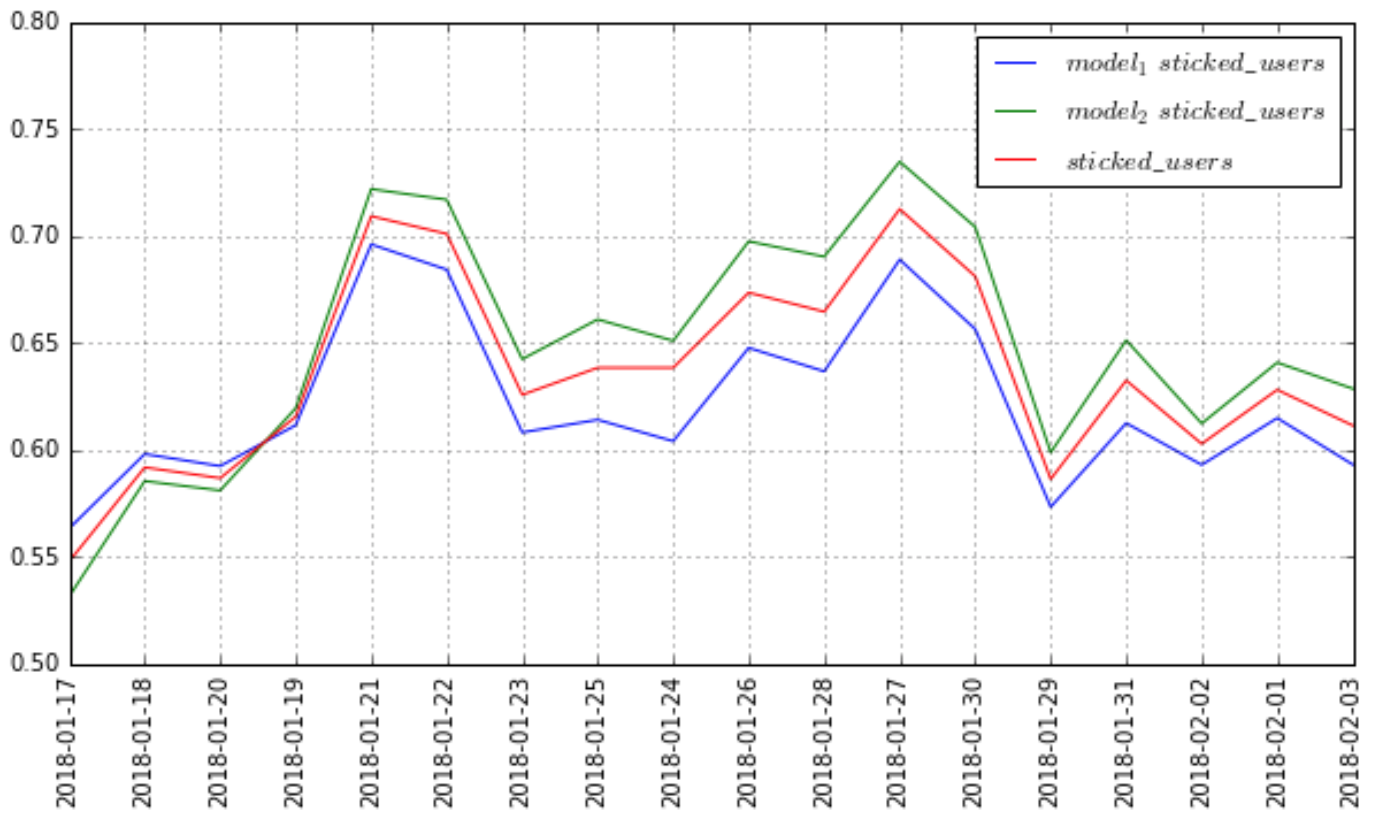
\includegraphics[height=6cm]{img1.png}

\par
\vspace{3mm}

Чем больше относительная разница между моделями - тем больше выгода использования оптимизатора из бейзлайна, что и ожидалось.
\par
\vspace{3mm}

На графике (2) - метрика оптимизаторов $optimizer\_metric(baseline)$
\par
\vspace{3mm}

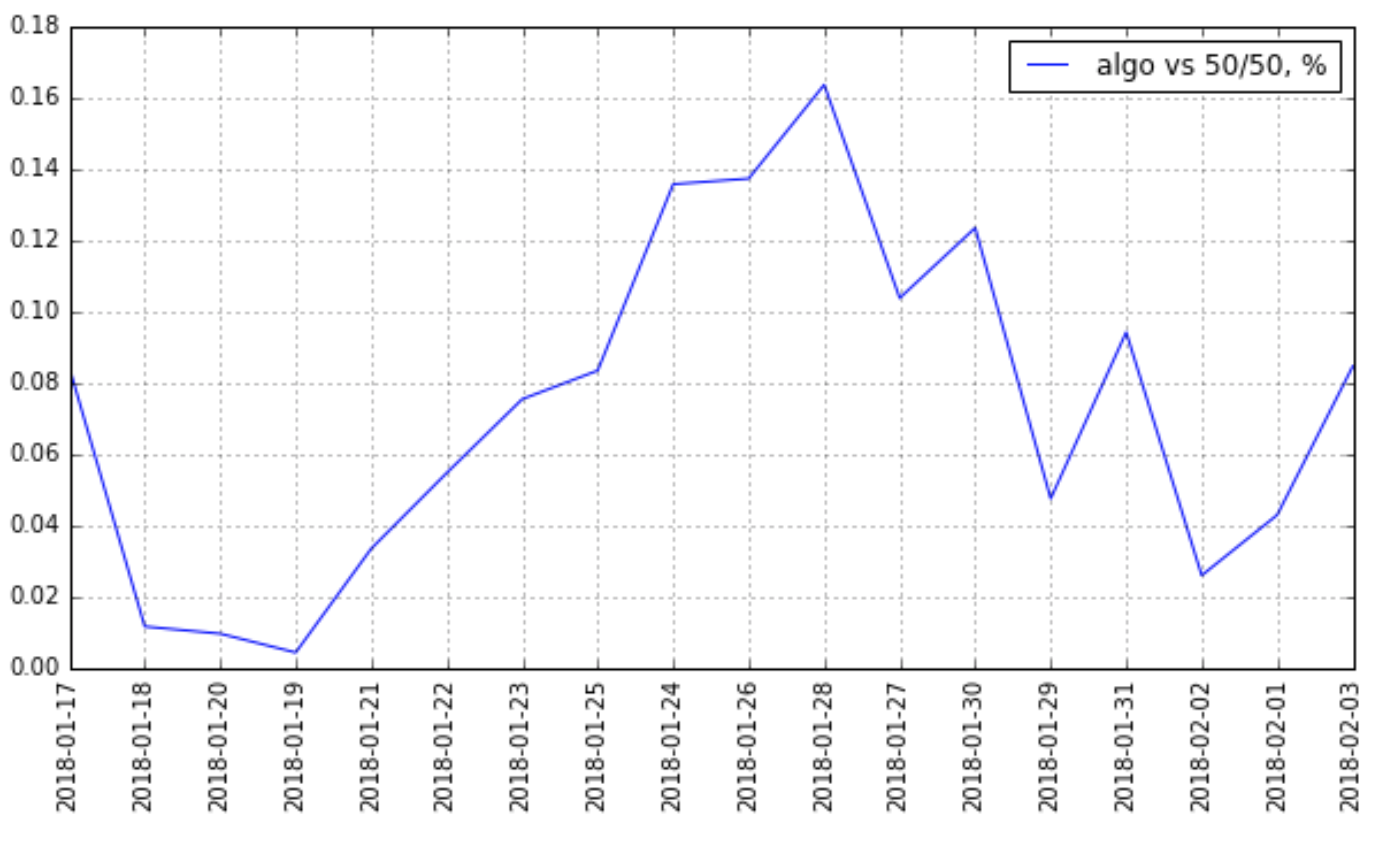
\includegraphics[height=6cm]{img2.png}
\par
\vspace{3mm}

Разница бейзлайна с простым А/Б-тестом совсем незначительная: порядка 0.1\%. Это происходит по причине того, что у двух моделей очень похожие конверсии, хотя одна из них стабильно немного лучше другой. Из-за маленькой разницы распределение весов по моделям близко к равномерному.

\par
\vspace{3mm}

\section{Эвристическая оптимизация с подбором новых моделей (TBD)}

\section{Методы оптимизации функций многих переменных из матанализа (TBD)}

\section{Оптимизация с помощью обучения с подкреплением (TBD)}

\section{Результаты и выводы (TBD)}


\section{Ссылки}

[1] p.86, \url{abitu.net/public/admin/mipt-conference/FPMI.pdf}


[2] \url{github.com/alexlokotochek/multiarmed-bandit}
\par
\vspace{3mm}



\end{document}
